\documentclass[12pt,a4paper]{report}

% -------- Packages --------
% NOTE: this document is compiled with pdfLaTeX. It previously required
% XeLaTeX for a native right-to-left Arabic abstract (via polyglossia +
% fontspec); that abstract has been removed, so the document no longer
% needs a Unicode-aware engine and uses the standard pdfLaTeX-era
% inputenc/fontenc/babel stack instead. The French abstract and any other
% French passage stays fully supported: babel's `french` module handles
% accented characters and French typographic/hyphenation rules under
% pdfLaTeX exactly as it would under XeLaTeX.
\usepackage[utf8]{inputenc}
\usepackage[T1]{fontenc}
\usepackage[french,main=english]{babel} % main document language: English

\usepackage{graphicx}
\usepackage{geometry}
\usepackage{setspace}
\usepackage{hyperref}
\usepackage{tocloft}
\usepackage{amsmath}
\usepackage{float}
\usepackage{longtable}
\usepackage{xcolor}
\usepackage{titlesec}
\usepackage{listings}
\usepackage{array}
\usepackage{acronym}
\usepackage[table]{xcolor}
\usepackage{tabularx}
\usepackage{tikz}
\usetikzlibrary{arrows.meta, positioning, fit, backgrounds}
\definecolor{ganttpink}{RGB}{255,192,192}
\definecolor{ganttgray}{RGB}{220,220,220}
\definecolor{codebg}{RGB}{245,245,245}

\geometry{top=2.5cm, bottom=2.5cm, left=2.5cm, right=2.5cm}

% Chapters I, II, III... instead of 1, 2, 3 (matches the requested outline).
\renewcommand{\thechapter}{\Roman{chapter}}

\lstset{
  basicstyle=\ttfamily\footnotesize,
  backgroundcolor=\color{codebg},
  frame=single,
  breaklines=true,
  columns=fullflexible,
  showstringspaces=false,
  captionpos=b,
}

\hypersetup{
  colorlinks=true,
  linkcolor=black,
  citecolor=black,
  urlcolor=blue,
  pdftitle={CompliaHub: Agentic GraphRAG Platform for Compliance Intelligence and Code Auditing},
  pdfauthor={Ahmed Amin Chabbah}
}

\begin{document}
\pagenumbering{gobble}
% ---------------- Cover Page (Page de garde) ----------------
\begin{titlepage}
\begin{center}
\noindent
\makebox[\textwidth][c]{%
  \raisebox{-0.4\height}{\includegraphics[scale=0.25]{images/insat2.jpg}}%
  \hfill
  \begin{minipage}{0.8\textwidth}
    \centering
    \small
    \textbf{REPUBLIC OF TUNISIA} \\
    Ministry of Higher Education and Scientific Research \\
    University of Carthage \\
    \textbf{National Institute of Applied Science and Technology (INSAT)}
  \end{minipage}%
  \hfill
  \raisebox{-0.4\height}{\includegraphics[scale=0.25]{images/ucar.png}}%
}

\vspace{0.5cm}
\noindent\rule{\textwidth}{0.5pt}
\vspace{1.5cm}

{\LARGE \textbf{Summer Internship Report}}\\[0.5cm]
\vspace{3mm}
\Large Completed as part of the 4\textsuperscript{th} year in Software Engineering at INSAT
\vspace{2.5mm}

\noindent\rule{\textwidth}{0.7pt} \\[2mm]
\LARGE \textbf{CompliaHub: Agentic GraphRAG Platform for Compliance Intelligence and Code Auditing}
\\\noindent\rule{\textwidth}{0.7pt}

\vspace{1.5cm}

\Large \textbf{Prepared by: Ahmed Amin Chabbah}\\[0.5cm]


\Large \textbf{Supervised by: Med Kamel Ben Hiba}\\[0.5cm]

\Large \textbf{Host Company: Nadas Group}\\[0.5cm]
\vspace{0.5cm}
\includegraphics[width=0.45\textwidth]{images/nadas_logo.png}\\[0.5cm]
\vspace{0.5cm}
\Large \textbf{Internship Period : 01 July - 31 August}\\[0.5cm]


\vfill

Academic Year: \textbf{2025 -- 2026}

\vspace{0.5cm}

\end{center}



\end{titlepage}

\clearpage
% --------- page signature ---------
\begin{titlepage}
\begin{center}
\noindent
\makebox[\textwidth][c]{%
  \raisebox{-0.4\height}{\includegraphics[scale=0.25]{images/insat2.jpg}}%
  \hfill
  \begin{minipage}{0.8\textwidth}
    \centering
    \small
    \textbf{REPUBLIC OF TUNISIA} \\
    Ministry of Higher Education and Scientific Research \\
    University of Carthage \\
    \textbf{National Institute of Applied Science and Technology (INSAT)}
  \end{minipage}%
  \hfill
  \raisebox{-0.4\height}{\includegraphics[scale=0.25]{images/ucar.png}}%
}

\vspace{0.5cm}
\noindent\rule{\textwidth}{0.5pt}
\vspace{1.2cm}

{\LARGE \textbf{Summer Internship Report}}\\[0.5cm]
\vspace{6mm}
\Large Completed as part of the 4\textsuperscript{th} year in Software Engineering at INSAT
\vspace{3mm}

\noindent\rule{\textwidth}{0.7pt} \\[2mm]
\LARGE \textbf{CompliaHub: Agentic GraphRAG Platform for Compliance Intelligence and Code Auditing}
\\\noindent\rule{\textwidth}{0.7pt}

\vspace{1.1cm}

\Large \textbf{Prepared by: Ahmed Amin Chabbah}\\[0.5cm]


\vspace{0.2cm}

\large \textbf{Host Company: Nadas Group}

\vspace{1.2cm}

\renewcommand{\arraystretch}{2.2}
\setlength{\tabcolsep}{18pt}
\begin{tabular}{|>{\centering\arraybackslash}m{7cm}|>{\centering\arraybackslash}m{7cm}|}
    \hline
    \small Company Supervisor:\par Mr. Med Kamel Ben Hiba & \small Internship Committee Evaluation \\
    [3cm] % space for signatures
    \hline
\end{tabular}
\renewcommand{\arraystretch}{1}

\vspace{0.9cm}

{\Large \textbf{Academic Year: 2025-- 2026}}

\vspace{0.5cm}



\end{center}
\end{titlepage}

% --------- Acknowledgment ---------
\chapter*{Acknowledgment}

\setstretch{1.2}
I would like to extend my deepest gratitude to my supervisor, Mr Med Kamel Ben Hiba, for his invaluable guidance, support, and encouragement throughout the duration of my internship. His expertise and insights have been instrumental in my learning and development.

I am profoundly grateful to the entire team at Nadas Group for providing me with this incredible opportunity and a conducive environment to grow professionally. The collaborative and innovative spirit of the organization has greatly enriched my internship experience.

Thank you all for your unwavering support and for making this internship a memorable and rewarding journey.

\clearpage

% ================================================================
% ABSTRACTS (FR / EN)
% ================================================================
\chapter*{Abstract}
\addcontentsline{toc}{chapter}{Abstract}

\section*{Résumé (Français)}
\begin{otherlanguage}{french}
Les équipes chargées de la conformité doivent répondre à des questions riches
en relations à travers plusieurs référentiels (ISO 42001, ISO 27001, RGPD) --
correspondances entre normes, analyse d'écarts, recherche de preuves d'audit
-- des questions que la recherche vectorielle classique traite mal, car elle
ignore la structure relationnelle du texte réglementaire. Ce rapport présente
\textbf{CompliaHub}, une plateforme développée durant un stage d'été de deux
mois chez Nadas Group, combinant une architecture \emph{GraphRAG} (recherche
vectorielle et parcours de graphe de connaissances) et une boucle
\emph{agentique} (planification, récupération, critique, réécriture) pour
répondre à ces questions avec citation systématique de la clause source.
Un second volet, le \emph{Compliance Scanner}, réutilise la même
infrastructure pour auditer un dépôt de code : des règles déterministes
détectent des non-conformités techniques (secrets, cryptographie faible,
fuites de données), qui sont ensuite cartographiées sur les contrôles de
l'Annexe A d'ISO/IEC 27001:2022, validées par un agent IA, puis obligatoirement
confirmées par une revue humaine avant tout statut positif -- jamais de
verdict de conformité généré automatiquement. Le rapport détaille la
méthodologie itérative adoptée, l'architecture technique (FastAPI, Next.js,
PostgreSQL, Neo4j, Qdrant, Celery), l'implémentation, la validation (511 tests
backend, 37 tests bout-en-bout frontend, un harnais d'évaluation fondé sur un
LLM-juge) ainsi que la stratégie de déploiement retenue, combinant Vercel pour
le frontend et une infrastructure conteneurisée persistante pour les services
avec état.
\end{otherlanguage}

\section*{Abstract (English)}
Compliance teams must answer relationship-heavy questions across multiple
standards (ISO 42001, ISO 27001, GDPR) -- cross-standard mapping, gap
analysis, audit-evidence lookup -- which plain vector search handles poorly,
since it ignores the relational structure of regulatory text. This report
presents \textbf{CompliaHub}, a platform built during a two-month summer
internship at Nadas Group, combining a \emph{GraphRAG} architecture (vector
search plus knowledge-graph traversal) with an \emph{agentic} loop (plan,
retrieve, critique, rewrite) to answer such questions with a citation back to
the exact source clause every time. A second initiative, the
\emph{Compliance Scanner}, reuses the same infrastructure to audit an
uploaded code repository: deterministic rules detect technical
non-compliance (secrets, weak cryptography, data leaks), which are then
mapped onto ISO/IEC 27001:2022 Annex A controls, validated by an AI agent,
and only ever confirmed by a mandatory human review before any positive
status is recorded -- never an automatically generated compliance verdict.
This report covers the iterative methodology adopted, the technical
architecture (FastAPI, Next.js, PostgreSQL, Neo4j, Qdrant, Celery), the
implementation, the validation performed (511 backend tests, 37 end-to-end
frontend tests, an LLM-judge evaluation harness), and the deployment
strategy adopted, combining Vercel for the frontend with a persistent
containerized infrastructure for the stateful services.

\clearpage

% ================================================================
% FRONT MATTER
% ================================================================
\pagenumbering{roman}

\tableofcontents
\clearpage

\listoffigures
\addcontentsline{toc}{chapter}{List of Figures}
\clearpage

\listoftables
\addcontentsline{toc}{chapter}{List of Tables}
\clearpage

\chapter*{List of Acronyms}
\addcontentsline{toc}{chapter}{List of Acronyms}
\begin{acronym}
\acro{AI}{Artificial Intelligence}
\acro{API}{Application Programming Interface}
\acro{AST}{Abstract Syntax Tree}
\acro{CI/CD}{Continuous Integration / Continuous Deployment}
\acro{CRUD}{Create, Read, Update, Delete}
\acro{CSS}{Cascading Style Sheets}
\acro{DB}{Database}
\acro{DOM}{Document Object Model}
\acro{ERD}{Entity-Relationship Diagram}
\acro{GDPR}{General Data Protection Regulation}
\acro{GRC}{Governance, Risk and Compliance}
\acro{HTTP}{Hypertext Transfer Protocol}
\acro{HTTPS}{Hypertext Transfer Protocol Secure}
\acro{ISO}{International Organization for Standardization}
\acro{JSON}{JavaScript Object Notation}
\acro{JWT}{JSON Web Token}
\acro{LLM}{Large Language Model}
\acro{NFR}{Non-Functional Requirement}
\acro{ORM}{Object-Relational Mapping}
\acro{PDF}{Portable Document Format}
\acro{PR}{Pull Request}
\acro{RAG}{Retrieval-Augmented Generation}
\acro{REST}{Representational State Transfer}
\acro{SaaS}{Software as a Service}
\acro{SAST}{Static Application Security Testing}
\acro{SSE}{Server-Sent Events}
\acro{UI}{User Interface}
\acro{UML}{Unified Modeling Language}
\acro{URL}{Uniform Resource Locator}
\acro{UX}{User Experience}
\acro{WCAG}{Web Content Accessibility Guidelines}
\end{acronym}
\clearpage

\pagenumbering{arabic}
\setcounter{page}{1}

% ================================================================
% GENERAL INTRODUCTION
% ================================================================
\chapter*{General Introduction}
\addcontentsline{toc}{chapter}{General Introduction}

Compliance work is, at its core, an information-retrieval problem dressed up
as a legal one. An analyst preparing for an ISO 27001 audit does not need a
generic summary of the standard -- they need the exact control that covers a
specific risk, the clause of the \ac{GDPR} that a given data flow must
satisfy, or every place in a codebase where a security control described on
paper is missing in practice. These questions are relationship-heavy by
nature: they span multiple documents, multiple standards, and multiple
levels of abstraction (a risk, a control, a piece of evidence), which is
precisely the shape of question that plain vector-similarity search handles
poorly, since embeddings capture semantic closeness but not the explicit
graph of references, mappings, and dependencies that regulatory text is built
from.

This report documents the design, implementation, and validation of
\textbf{CompliaHub}, a platform built to close that gap on two fronts. The
first is a conversational compliance-intelligence engine that answers
natural-language questions about ingested standards (ISO 42001, ISO 27001,
\ac{GDPR}) using a \ac{RAG} architecture combining vector search with a
knowledge-graph traversal layer, orchestrated by an agentic loop capable of
planning, retrieving, critiquing its own evidence, and retrying. The second,
the \emph{Compliance Scanner}, reuses the same backend to turn an uploaded
source-code repository into evidence-grounded compliance findings, mapped
onto real ISO 27001 Annex A controls, with every positive verdict requiring
mandatory human review -- a deliberate refusal to let automation alone ever
certify anything.

The remainder of this report is organized as follows. Chapter~I sets the
general framework: context, motivation, objectives, and the methodology and
planning adopted for a two-month, single-developer internship. Chapter~II
covers the study and specification phase: the state of the art, the concepts
this project builds on, and a full requirements study. Chapter~III presents
the system's architecture and design, both at a technology-agnostic level
and with the concrete stack chosen. Chapter~IV describes the implementation:
the development environment, the key algorithms, the difficulties
encountered, and the resulting user interfaces. Chapter~V reports on the
testing and validation performed, and Chapter~VI concludes with a summary of
the work, its contributions, and directions for future improvement.

% ================================================================
% CHAPTER I -- GENERAL FRAMEWORK
% ================================================================
\chapter{General Framework}

\section{General Context}

Organizations subject to information-security and data-protection
regulation are increasingly expected to demonstrate compliance against
several overlapping standards at once. ISO/IEC 27001 (information security
management), ISO/IEC 42001 (AI management systems), and the \ac{GDPR} share
substantial conceptual overlap -- risk assessment, access control,
data-retention obligations -- but no shared vocabulary or shared tooling.
In practice, compliance analysts still work from static documents, and
engineering teams verify technical controls manually, with no direct,
evidence-linked path between "what the standard requires" and "what the
codebase actually does."

\section{Motivation and Problem Statement}

Compliance teams need to answer relationship-heavy questions across ISO
42001, ISO 27001, and \ac{GDPR}: cross-standard mapping, control mapping,
gap analysis, and audit-evidence lookup. Plain vector search handles these
poorly because it retrieves passages that are \emph{semantically} similar to
a query, not passages that are \emph{structurally connected} to it through
the standard's own network of clauses, controls, and cross-references. On
the engineering side, existing static-analysis tools flag technical issues
(secrets, weak cryptography, insecure configuration) without ever expressing
\emph{which regulatory requirement} that issue relates to, leaving the
translation from "a scanner found this" to "this satisfies (or fails)
control X" entirely manual.

\section{Project Objectives}

The project set out to satisfy the following, concrete success criteria:

\begin{itemize}
  \item Answer multi-hop compliance questions correctly, with a citation
        back to the exact source clause or article for every claim made.
  \item Keep response latency proportionate to query complexity: a simple,
        single-clause lookup should resolve in a few seconds, while a full
        agentic research loop may reasonably take longer.
  \item Support incremental ingestion -- adding one new standard should
        never require reprocessing the entire corpus from scratch.
  \item Extend the same retrieval infrastructure to a second, standalone
        use case: auditing an uploaded codebase for technical compliance
        evidence, always expressed through an explicit, six-value evidence
        vocabulary (\texttt{VERIFIED}, \texttt{PARTIALLY\_VERIFIED},
        \texttt{NOT\_VERIFIED}, \texttt{POTENTIAL\_NON\_COMPLIANCE},
        \texttt{NOT\_APPLICABLE}, \texttt{REQUIRES\_HUMAN\_REVIEW}) --
        never a bare "compliant" / "non-compliant" verdict, and never one
        asserted by automation alone.
\end{itemize}

Two explicit non-goals were set from the outset, to keep the scope
proportionate to a two-month internship: multi-tenant \ac{SaaS} support and
real-time collaborative editing were both deliberately excluded from this
first version, as was support for non-English documents and file types
beyond \ac{PDF}/DOCX.

\section{Report Outline}

Chapter~I (this chapter) frames the project. Chapter~II covers the state of
the art and the requirements specification. Chapter~III presents the
system's architecture and design. Chapter~IV details the implementation.
Chapter~V reports on testing and validation. Chapter~VI concludes with a
summary of contributions and future directions, followed by annexes and a
bibliography.

\section{Methodology}

Because this was a single-developer internship rather than a multi-person
team project, a lightweight, Scrum-inspired methodology was adopted rather
than a full ceremony-driven Scrum process. The project's own roadmap
(\texttt{GraphRAG-Agentic-RAG-Roadmap.md}) decomposes the work into 18
sequential phases across two parallel tracks -- 9 platform phases (ingestion
through scaling and hardening) and 9 Compliance Scanner phases (rule-based
detection through automated remediation) -- each of which was treated as one
short, self-contained sprint. Every phase followed the same three-step
cycle:

\begin{enumerate}
  \item \textbf{Plan.} A phase document is written \emph{before} any code
        is written, capturing the goal, the concepts that need to be
        learned, and the components to be built.
  \item \textbf{Build and verify live.} The phase is implemented, then
        verified against the actual running stack (Docker Compose services,
        a real backend process, a real browser) rather than against mocks
        alone -- a discipline adopted directly in response to an early
        lesson of this project: mocked tests alone missed real
        infrastructure and hydration bugs that only a live run surfaced.
  \item \textbf{Update the document in place.} The same phase document is
        updated afterward with what was actually built, the bugs found
        along the way, and how each claim was verified -- becoming the
        as-built reference for that layer of the system, and playing the
        role a sprint retrospective would in a team setting.
\end{enumerate}

\ac{CI/CD} reinforced this discipline automatically: every push to the main
branch and every pull request triggers a GitHub Actions pipeline that lints
and tests both the backend (\texttt{ruff}, \texttt{pytest}) and the frontend
(\texttt{eslint}, a production build), so a phase was never considered
"done" while the pipeline was red.

\section{Project Planning}

The two-month internship (01 July -- 31 August) was organized into nine
weekly work packages, grouping the 18 roadmap phases into coherent blocks of
related work. Table~\ref{tab:gantt} summarizes the planning actually
followed.

\begin{table}[H]
\centering
\caption{Project planning (work packages by week)}
\label{tab:gantt}
\renewcommand{\arraystretch}{1.3}
\begin{tabularx}{\textwidth}{@{}l*{9}{>{\centering\arraybackslash}X}@{}}
\toprule
\textbf{Work package} & \textbf{W1} & \textbf{W2} & \textbf{W3} & \textbf{W4} & \textbf{W5} & \textbf{W6} & \textbf{W7} & \textbf{W8} & \textbf{W9} \\
\midrule
Setup \& ingestion pipeline & \cellcolor{ganttpink} & \cellcolor{ganttpink} & & & & & & & \\
Vector \& graph retrieval & & \cellcolor{ganttpink} & \cellcolor{ganttpink} & & & & & & \\
Agentic orchestration \& frontend v1 & & & \cellcolor{ganttpink} & \cellcolor{ganttpink} & & & & & \\
Evaluation harness \& scaling & & & & \cellcolor{ganttpink} & \cellcolor{ganttpink} & & & & \\
Scanner: rules \& ISO 27001 mapping & & & & & \cellcolor{ganttpink} & \cellcolor{ganttpink} & & & \\
Scanner: AI validation \& review & & & & & & \cellcolor{ganttpink} & \cellcolor{ganttpink} & & \\
Scanner: reports \& remediation & & & & & & & \cellcolor{ganttpink} & \cellcolor{ganttpink} & \\
Frontend redesign (full product) & & & & & & & & \cellcolor{ganttpink} & \cellcolor{ganttpink} \\
Testing, deployment \& report writing & & & & & & & & \cellcolor{ganttgray} & \cellcolor{ganttpink} \\
\bottomrule
\end{tabularx}
\end{table}

Work packages overlap by one week by design: each new package's first days
were spent validating the previous one live before building on top of it,
matching the "verify before you build further" discipline described above.

% ================================================================
% CHAPTER II -- STUDY AND SPECIFICATION
% ================================================================
\chapter{Study and Specification Phase}

\section{State of the Art and Study of Existing Solutions}

\subsection{Research and Existing Solutions}

Retrieval-augmented generation has become the standard approach for
grounding \acp{LLM} in a private document corpus, but plain vector-similarity
\ac{RAG} treats every chunk of text as an independent unit, which discards
exactly the relational structure -- cross-references, control mappings,
hierarchical clause structure -- that compliance documents are built from.
Microsoft's GraphRAG approach~\cite{edge2024graphrag} addresses this by
building an explicit knowledge graph over extracted entities and
relationships, then combining graph traversal with vector retrieval;
alternative graph-augmented designs (LightRAG, RAPTOR, HippoRAG) explore
similar territory with different indexing and summarization strategies. On
the tooling side, existing \ac{SAST} scanners (pattern- and \ac{AST}-based
tools in the same family as Bandit or Semgrep) reliably detect technical
issues in source code, but report them without any link to a regulatory
requirement, and commercial \ac{GRC} platforms typically track compliance
status through manually maintained checklists rather than generating
evidence directly from a standard's own text or from a live scan of the
system it governs.

\subsection{Technologies, Methods, and Tools Used in the Domain}

The current \ac{RAG} tooling landscape offers several building blocks
this project draws on directly: dedicated vector databases (Qdrant, among
others) for approximate nearest-neighbor search over embeddings; graph
databases (Neo4j) for storing and traversing an explicit entity-relationship
graph; community-detection algorithms (the Leiden algorithm) for clustering
a knowledge graph into coherent topical communities; cross-encoder reranking
models to refine an initial vector-search result set; and agent-orchestration
frameworks (LangGraph, among others) for building multi-step, stateful
LLM-driven control flows rather than a single prompt-response call.

\subsection{Limitations of Existing Solutions}

\begin{itemize}
  \item Plain vector \ac{RAG} cannot reliably answer cross-standard mapping
        or multi-hop questions, because nothing in the index represents the
        explicit relationships between clauses.
  \item Static-analysis scanners produce technical findings with no
        regulatory context, leaving the mapping from "code issue" to
        "control satisfied or violated" entirely manual.
  \item Commercial \ac{GRC} platforms depend on manually entered evidence
        and checklists, and cannot generate a compliance-evidence report
        directly from a live codebase scan.
  \item None of the above combine evidence retrieval, technical scanning,
        and a mandatory human-in-the-loop verification step in one
        traceable pipeline.
\end{itemize}

\section{Basic Concepts}

\textbf{\ac{CI/CD}.} Continuous Integration/Continuous Deployment automates
the build, lint, and test cycle on every code change; this project's
GitHub Actions pipeline (\texttt{.github/workflows/ci.yml}) runs the backend
test suite (\texttt{ruff}, \texttt{pytest}) and the frontend lint/build
(\texttt{eslint}, \texttt{pnpm build}) on every push and pull request.

\textbf{Cloud and containers.} The local development stack is fully
containerized via Docker Compose (PostgreSQL, Redis, Neo4j, Qdrant, MinIO,
and three role-scoped Celery workers), which guarantees the same
infrastructure runs identically on any machine and maps directly onto a
containerized production deployment.

\textbf{\ac{LLM}, \ac{RAG}, and agentic \ac{RAG}.} A \ac{LLM} generates text
conditioned on a prompt; \ac{RAG} augments that prompt with content
retrieved from an external corpus rather than relying solely on the model's
training data; an \emph{agentic} \ac{RAG} loop goes further, letting the
model itself decide, across multiple steps, how to plan a retrieval
strategy, critique the evidence it retrieved, and retry if that evidence is
judged insufficient.

\textbf{Vector and graph databases.} A vector database indexes numerical
embeddings of text for approximate nearest-neighbor search (semantic
similarity); a graph database stores explicit nodes and typed relationships
and supports traversal queries (e.g. "every node reachable from this one
within two hops"), which is the data model that makes cross-standard mapping
and multi-hop questions answerable at all.

\textbf{Deployment models (serverless/edge).} A serverless-style deployment
platform (such as Vercel, used for this project's frontend -- see
Chapter~IV) builds and deploys an application automatically on every push,
serving it from a global edge network with zero server management from the
developer, in contrast to a persistent, stateful backend that must run
continuously and therefore needs a traditional container host.

\section{Specification}

\subsection{Needs Study}

\subsubsection{Identification of Actors}

\begin{itemize}
  \item \textbf{Compliance analyst.} Asks natural-language questions about
        the ingested standards and reads cited answers.
  \item \textbf{Security/compliance auditor.} Uploads a codebase for
        scanning and inspects the resulting findings.
  \item \textbf{Human reviewer.} Confirms or rejects a finding with a
        written justification -- the only actor able to assert a positive
        compliance status.
  \item \textbf{Platform operator.} Ingests new standards documents,
        monitors the pipeline, and manages access control and rate limits.
\end{itemize}

\begin{figure}[H]
\centering
\begin{tikzpicture}[
  actor/.style={draw, rectangle, rounded corners, minimum width=3.1cm, minimum height=0.9cm, align=center, font=\footnotesize},
  usecase/.style={draw, ellipse, minimum width=4.3cm, minimum height=0.8cm, align=center, font=\footnotesize},
  >=Latex
]
  \node[actor] (analyst) at (0,4.5) {Compliance\\Analyst};
  \node[actor] (auditor) at (0,2.5) {Security/Compliance\\Auditor};
  \node[actor] (reviewer) at (0,0.5) {Human\\Reviewer};
  \node[actor] (operator) at (0,-1.5) {Platform\\Operator};

  \node[usecase] (ask)      at (5.5,5.3) {Ask a compliance question};
  \node[usecase] (converse) at (5.5,4.2) {Continue a conversation};
  \node[usecase] (upload)   at (5.5,3.1) {Upload a codebase (.zip)};
  \node[usecase] (findings) at (5.5,2.0) {Browse scan findings};
  \node[usecase] (validate) at (5.5,0.9) {Trigger AI validation / remediation};
  \node[usecase] (review)   at (5.5,-0.2) {Submit a human review};
  \node[usecase] (report)   at (5.5,-1.3) {Generate a printable report};
  \node[usecase] (ingest)   at (5.5,-2.4) {Ingest a standard document};

  \draw[->] (analyst) -- (ask);
  \draw[->] (analyst) -- (converse);
  \draw[->] (auditor) -- (upload);
  \draw[->] (auditor) -- (findings);
  \draw[->] (auditor) -- (validate);
  \draw[->] (auditor) -- (report);
  \draw[->] (reviewer) -- (review);
  \draw[->] (operator) -- (ingest);
\end{tikzpicture}
\caption{General use-case diagram of the CompliaHub platform}
\label{fig:usecase}
\end{figure}

\subsubsection{Functional Requirements}

\begin{itemize}
  \item Ingest a \ac{PDF}/DOCX standard, chunk it, embed it, and extract its
        entities and relationships into a knowledge graph.
  \item Answer a natural-language question, classified and routed to
        vector search, graph traversal, or a full agentic loop, with a
        citation to the exact source clause and, for multi-turn
        conversations, memory of prior turns.
  \item Upload a repository archive and run deterministic security,
        \ac{GDPR}, and AI-governance rule engines against it with zero
        \ac{LLM} calls at detection time.
  \item Map every resulting finding onto real ISO/IEC 27001:2022 Annex A
        control identifiers.
  \item Trigger an agentic \ac{RAG} pass that grounds a finding against the
        ingested standards and reports a reasoned assessment, without ever
        changing the finding's status itself.
  \item Record a human review decision (with a mandatory written
        justification) as the only mechanism able to mark a finding
        verified.
  \item Suggest a concrete unified-diff code fix for a finding, without
        ever applying it automatically.
  \item Generate a printable, per-scan evidence report broken down by
        severity, status, and framework, with no aggregate compliance score
        anywhere.
  \item Delete an ingested document and rebuild the knowledge graph from
        the documents that remain.
  \item Run an evaluation harness that scores a reviewed question set on
        faithfulness, answer relevance, context precision, and context
        recall.
\end{itemize}

\subsubsection{Non-Functional Requirements}

\begin{itemize}
  \item \textbf{Performance.} A simple, single-clause query should resolve
        in a few seconds; a full agentic research loop may reasonably take
        longer, proportionate to the depth of retrieval it performs.
  \item \textbf{Scalability / incremental updates.} Adding one new document
        must not require reprocessing the entire corpus.
  \item \textbf{Security.} Opt-in \ac{API} key authentication on mutating
        routes, and Redis-backed rate limiting on the query endpoints
        (20 requests/minute by default).
  \item \textbf{Accessibility.} \ac{WCAG} AA color-contrast compliance
        (verified by an automated test reading the live computed styles,
        not a static table), full keyboard operability, and
        \texttt{prefers-reduced-motion} support throughout the interface.
  \item \textbf{Multi-theme support.} A real light/dark theme toggle,
        persisted across sessions, rather than following only the
        operating system's preference.
  \item \textbf{Print fidelity.} The evidence report must render correctly
        when printed, in either theme.
  \item \textbf{Maintainability.} Every phase of the build is documented
        before and after implementation, and the full test suite (511
        backend tests, 37 frontend end-to-end tests at the time of writing)
        must stay green on every change.
  \item \textbf{Disclosed limitations, by design.} Single-language (English)
        documents and no multi-tenant isolation in this version -- explicit
        non-goals rather than silent gaps.
\end{itemize}

% ================================================================
% CHAPTER III -- ARCHITECTURE AND DESIGN
% ================================================================
\chapter{Planning: Architecture and Conception}

\section{General (Technology-Agnostic) Architecture}

The system follows a layered, client-server architecture: a presentation
layer (the web frontend), an orchestration layer (the backend \ac{API}), a
retrieval layer split between vector and graph search, and a persistence
layer split by data shape (relational metadata, vector embeddings, graph
structure, object storage, and a cache/queue). Figure~\ref{fig:arch-generic}
shows this decomposition independently of any specific technology.

\begin{figure}[H]
\centering
\begin{tikzpicture}[
  box/.style={draw, rectangle, rounded corners, minimum width=8.6cm, minimum height=0.9cm, align=center, font=\footnotesize},
  smallbox/.style={draw, rectangle, rounded corners, minimum width=2.7cm, minimum height=0.9cm, align=center, font=\footnotesize},
  >=Latex
]
  \node[box] (front) at (0,6) {Presentation Layer\\(Web Frontend)};
  \node[box] (api)   at (0,4.6) {Orchestration Layer\\(Backend API)};

  \node[smallbox] (classifier) at (-3,3.1) {Query Classifier};
  \node[smallbox] (agent)      at (0,3.1)  {Agentic Loop};
  \node[smallbox] (ingestion)  at (3,3.1)  {Ingestion Pipeline};

  \node[box] (retrieval) at (0,1.6) {Retrieval Layer -- Vector Search \& Graph Traversal};

  \node[smallbox] (relational) at (-3,0.1) {Relational Store};
  \node[smallbox] (cache)      at (0,0.1)  {Cache \& Queue};
  \node[smallbox] (object)     at (3,0.1)  {Object Storage};

  \draw[<->] (front) -- (api);
  \draw[->] (api) -- (classifier);
  \draw[->] (api) -- (agent);
  \draw[->] (api) -- (ingestion);
  \draw[->] (classifier) -- (retrieval);
  \draw[->] (agent) -- (retrieval);
  \draw[->] (ingestion) -- (retrieval);
  \draw[->] (retrieval) -- (relational);
  \draw[->] (retrieval) -- (cache);
  \draw[->] (retrieval) -- (object);
\end{tikzpicture}
\caption{Technology-agnostic architecture}
\label{fig:arch-generic}
\end{figure}

\subsection{Architecture Type}

The backend is a \textbf{modular monolith}, not a microservices system:
a single FastAPI application exposes every route, but its internal modules
(query orchestration, ingestion, scanner rule engines, evaluation) are
cleanly separated and independently testable, and asynchronous work is
split across three role-scoped Celery workers (\texttt{worker-ingestion},
\texttt{worker-vector}, \texttt{worker-graph}) rather than one general-purpose
queue. This is a deliberate, honest classification: the system is
client-server and layered, with role-based task distribution, rather than a
set of independently deployable microservices each owning their own
database.

\subsection{Database Type}

The persistence layer is \textbf{polyglot} by design, each store chosen for
the shape of data it holds: PostgreSQL (relational) for metadata, job state,
and provenance -- using the \texttt{ltree} extension to model clause
hierarchy; Qdrant (vector) for embedding similarity search; Neo4j (graph)
for the extracted entity-relationship graph and community structure; MinIO
(S3-compatible object storage) for raw uploaded documents; and Redis for
caching, the Celery broker/result backend, and rate-limit counters.

\section{Architecture with Technologies}

Figure~\ref{fig:arch-tech} repeats the same decomposition, naming the actual
technology chosen at each layer; Table~\ref{tab:techstack} lists the full
stack.

\begin{figure}[H]
\centering
\begin{tikzpicture}[
  box/.style={draw, rectangle, rounded corners, minimum width=8.6cm, minimum height=1.1cm, align=center, font=\footnotesize},
  smallbox/.style={draw, rectangle, rounded corners, minimum width=2.8cm, minimum height=1.1cm, align=center, font=\footnotesize},
  >=Latex
]
  \node[box] (front) at (0,6.6) {Next.js 16 / React 19\\(Chat + Scanner UI)};
  \node[box] (api)   at (0,5.0) {FastAPI (Python 3.12)};

  \node[smallbox] (classifier) at (-3,3.3) {Classifier\\(Gemini)};
  \node[smallbox] (agent)      at (0,3.3)  {LangGraph\\Agent Loop};
  \node[smallbox] (ingestion)  at (3,3.3)  {Docling +\\Celery};

  \node[box] (retrieval) at (0,1.6) {Qdrant (vector) \quad + \quad Neo4j (graph)};

  \node[smallbox] (relational) at (-3,0.1) {PostgreSQL};
  \node[smallbox] (cache)      at (0,0.1)  {Redis + Celery};
  \node[smallbox] (object)     at (3,0.1)  {MinIO (S3)};

  \draw[<->] (front) -- (api);
  \draw[->] (api) -- (classifier);
  \draw[->] (api) -- (agent);
  \draw[->] (api) -- (ingestion);
  \draw[->] (classifier) -- (retrieval);
  \draw[->] (agent) -- (retrieval);
  \draw[->] (ingestion) -- (retrieval);
  \draw[->] (retrieval) -- (relational);
  \draw[->] (retrieval) -- (cache);
  \draw[->] (retrieval) -- (object);
\end{tikzpicture}
\caption{Architecture with the technologies actually used}
\label{fig:arch-tech}
\end{figure}

\begin{table}[H]
\centering
\caption{Technology stack}
\label{tab:techstack}
\begin{tabularx}{\textwidth}{@{}l X@{}}
\toprule
\textbf{Layer} & \textbf{Choice} \\
\midrule
Backend \ac{API} & FastAPI (Python 3.12, \texttt{uv}-managed) \\
Frontend & Next.js 16 / React 19 (TypeScript, Tailwind CSS v4, \texttt{pnpm}) \\
Relational database & PostgreSQL (metadata, job state; \texttt{ltree} for clause hierarchy) \\
Vector database & Qdrant \\
Graph database & Neo4j \\
Cache / task queue & Redis + Celery \\
Object storage & MinIO (S3-compatible) \\
Document parsing & Docling (structure-aware \ac{PDF}/DOCX) \\
Embeddings & Voyage AI (\texttt{voyage-law-2}) \\
Reranking & Cohere Rerank (\texttt{rerank-v3.5}) \\
Answer generation \& extraction & Google Gemini (\texttt{gemini-3.1-flash-lite}) \\
Community detection & \texttt{python-igraph} + \texttt{leidenalg} (Leiden algorithm) \\
Agent orchestration & LangGraph \\
Evaluation & Custom Gemini LLM-judge harness \\
\ac{CI/CD} & GitHub Actions \\
Containerization & Docker / Docker Compose \\
\bottomrule
\end{tabularx}
\end{table}

\section{Conception}

\subsection{Sequence Diagram -- Answering a Compliance Question}

Figure~\ref{fig:sequence} traces a single question from the user interface
to a cited answer, showing the classifier's routing decision and the
agentic loop's retrieve/critique cycle when a question requires it.

\begin{figure}[H]
\centering
\begin{tikzpicture}[font=\footnotesize, >=Latex]
  \def\ux{0} \def\fx{3.2} \def\bx{6.4} \def\lx{9.8}
  \node at (\ux,8.6) {User};
  \node at (\fx,8.6) {Frontend};
  \node at (\bx,8.6) {Backend};
  \node at (\lx,8.6) {Retrieval / LLM};

  \draw[dashed] (\ux,8.3) -- (\ux,0);
  \draw[dashed] (\fx,8.3) -- (\fx,0);
  \draw[dashed] (\bx,8.3) -- (\bx,0);
  \draw[dashed] (\lx,8.3) -- (\lx,0);

  \draw[->] (\ux,7.8) -- (\fx,7.8) node[midway, above] {1. asks question};
  \draw[->] (\fx,7.2) -- (\bx,7.2) node[midway, above] {2. POST /query/stream};
  \draw[->] (\bx,6.6) -- (\lx,6.6) node[midway, above] {3. classify query};
  \draw[->] (\lx,6.0) -- (\bx,6.0) node[midway, above] {4. category};
  \draw[->] (\bx,5.4) -- (\lx,5.4) node[midway, above] {5. retrieve (vector/graph)};
  \draw[->] (\lx,4.8) -- (\bx,4.8) node[midway, above] {6. evidence chunks};
  \draw[->] (\bx,4.2) -- (\lx,4.2) node[midway, above] {7. critique evidence};
  \draw[->,dashed] (\lx,3.6) -- (\bx,3.6) node[midway, above] {8. retry retrieval if insufficient};
  \draw[->] (\bx,3.0) -- (\lx,3.0) node[midway, above] {9. generate answer};
  \draw[->] (\lx,2.4) -- (\bx,2.4) node[midway, above] {10. streamed tokens};
  \draw[->] (\bx,1.8) -- (\fx,1.8) node[midway, above] {11. SSE: status + tokens};
  \draw[->] (\fx,1.2) -- (\ux,1.2) node[midway, above] {12. rendered answer + citations};
\end{tikzpicture}
\caption{Sequence diagram: answering a compliance question}
\label{fig:sequence}
\end{figure}

\subsection{Conceptual Model -- Scanner Finding Lifecycle}

Figure~\ref{fig:findinglifecycle} shows the conceptual relationships between
a scan, its findings, the evidence accumulated on each finding (rule output,
\ac{AI} validation, remediation suggestions), and the human reviews that are
the only mechanism able to assert a positive status.

\begin{figure}[H]
\centering
\begin{tikzpicture}[
  cls/.style={draw, rectangle, rounded corners, minimum width=3.4cm, align=left, font=\footnotesize},
  >=Latex
]
  \node[cls] (scan) at (0,4) {\textbf{Scan}\\repository, languages,\\pipeline status};
  \node[cls] (finding) at (4.5,4) {\textbf{Finding}\\severity, category,\\rule\_id, status};
  \node[cls] (evidence) at (9,5.4) {\textbf{Evidence}\\rule output / AI\\validation / diff};
  \node[cls] (review) at (9,2.6) {\textbf{Review}\\reviewer, decision,\\justification};
  \node[cls, minimum width=8.5cm] (status) at (4.5,0.5) {\textbf{Status vocabulary}: VERIFIED, PARTIALLY\_VERIFIED,\\ NOT\_VERIFIED, POTENTIAL\_NON\_COMPLIANCE,\\ NOT\_APPLICABLE, REQUIRES\_HUMAN\_REVIEW};

  \draw[->] (scan) -- node[above, font=\scriptsize]{1..*} (finding);
  \draw[->] (finding) -- node[above, font=\scriptsize]{0..*} (evidence);
  \draw[->] (finding) -- node[right, font=\scriptsize]{0..*} (review);
  \draw[->] (finding) -- (status);
\end{tikzpicture}
\caption{Conceptual model: the scanner finding lifecycle}
\label{fig:findinglifecycle}
\end{figure}

% ================================================================
% CHAPTER IV -- IMPLEMENTATION
% ================================================================
\chapter{Phase de Réalisation (Implementation)}

\section{Development Environment}
\label{sec:devenv}

\begin{table}[H]
\centering
\caption{Development environment}
\label{tab:devenv}
\begin{tabularx}{\textwidth}{@{}l X@{}}
\toprule
\textbf{Category} & \textbf{Tools} \\
\midrule
Languages & Python 3.12, TypeScript 5 \\
Backend framework & FastAPI, SQLAlchemy, Alembic, Celery \\
Frontend framework & Next.js 16 (App Router), React 19, Tailwind CSS v4 \\
Package managers & \texttt{uv} (backend), \texttt{pnpm} (frontend) \\
Version control & Git / GitHub \\
Containerization & Docker, Docker Compose \\
\ac{CI/CD} & GitHub Actions (lint + test on every push/PR) \\
Backend testing & \texttt{pytest}, \texttt{ruff} \\
Frontend testing & Playwright (end-to-end), ESLint \\
\bottomrule
\end{tabularx}
\end{table}

\section{Deployment Strategy}

The system is deliberately deployed as two separate concerns rather than
as one unit, following directly from the architectural classification made
in Chapter~III: a stateless presentation layer and a stateful backend with
five persistent data services behind it.

\textbf{Frontend -- Vercel.} The Next.js frontend is deployed on
\textbf{Vercel}~\cite{vercel}, the platform built by the maintainers of
Next.js itself, chosen for four concrete reasons directly relevant to this
project:

\begin{itemize}
  \item \textbf{Zero-configuration, framework-native builds.} Vercel
        detects a Next.js project automatically and builds/deploys it with
        no custom pipeline of its own to write or maintain.
  \item \textbf{Git-integrated continuous deployment.} Every push to the
        main branch triggers an automatic production deployment, and every
        pull request gets its own disposable preview \ac{URL} -- extending
        the existing GitHub Actions pipeline (which already lints and
        builds the frontend on every push/\ac{PR}, see
        Table~\ref{tab:devenv}) with an actual, reviewable deployed
        environment per change, rather than lint/build success alone.
  \item \textbf{Global edge network and automatic \ac{HTTPS}.} Static
        assets and server-rendered pages are served from an edge network
        close to the visitor, with certificate management handled
        automatically -- infrastructure this project would otherwise have
        to configure and maintain by hand.
  \item \textbf{Configuration via environment variables.} The single
        public configuration point the frontend needs, its backend origin
        (\texttt{NEXT\_PUBLIC\_API\_URL}), is set as a Vercel project
        environment variable rather than hardcoded, so the same build can
        point at a staging or production backend without a code change.
\end{itemize}

\textbf{Backend and data plane -- persistent containers, not Vercel.} The
backend and its five stateful services (PostgreSQL, Neo4j, Qdrant, Redis,
MinIO) and three Celery workers are deliberately \emph{not} deployed to
Vercel: Vercel's execution model is built around short-lived serverless
functions with bounded execution time and no persistent local process
state, which is fundamentally incompatible with a long-running Celery
worker, a stateful database connection pool, or a graph database that must
keep its data resident between requests. These are instead deployed using
the same Docker Compose definition already used for local development
(Section~\ref{sec:devenv}), pointed at a persistent container
host, so that the exact same service topology verified throughout
development is what actually runs in production -- deliberately avoiding a
second, divergent "production" infrastructure definition.

\textbf{Resulting split.} Table~\ref{tab:deployment} summarizes the adopted
deployment split. This is presented as the deployment strategy \emph{adopted
for this project going forward}: at the time of writing, the frontend's
Vercel deployment is the immediate, concrete target, while the backend
continues to run on the same containerized stack verified throughout
development, consistent with the project's own discipline of only claiming
what has actually been verified.

\begin{table}[H]
\centering
\caption{Deployment split by component}
\label{tab:deployment}
\begin{tabularx}{\textwidth}{@{}l X l@{}}
\toprule
\textbf{Component} & \textbf{Platform} & \textbf{Rationale} \\
\midrule
Next.js frontend & Vercel & Stateless, framework-native, benefits directly from edge delivery and preview deployments \\
FastAPI backend & Containerized host (Docker Compose) & Long-running process, stateful connections \\
PostgreSQL, Neo4j, Qdrant, Redis, MinIO & Containerized host (Docker Compose) & Persistent data services, incompatible with a serverless execution model \\
Celery workers (ingestion / vector / graph) & Containerized host (Docker Compose) & Long-running background processes \\
\bottomrule
\end{tabularx}
\end{table}

\section{Code Description and Key Algorithms}
\label{sec:code-description}

\textbf{Ingestion pipeline.} An uploaded \ac{PDF}/DOCX is parsed by Docling
into a structure-aware document tree, chunked, embedded (Voyage), and passed
to an extraction stage where Gemini identifies entities and relationships,
which are then resolved and loaded into the Neo4j graph; the Leiden
algorithm subsequently clusters the graph into topical communities used by
the graph-retrieval path.

\textbf{Query orchestration.} An incoming question is first classified into
a routing category (a direct vector lookup, a graph traversal, or a full
agentic loop) by a lightweight Gemini call. The agentic path, built on
LangGraph, executes a plan/retrieve/critique/rewrite cycle: it plans a
retrieval strategy, retrieves evidence, critiques whether that evidence is
sufficient to answer the question, and -- if not -- rewrites the query and
retries, up to a bounded number of iterations, before generating a final,
streamed, citation-carrying answer.

\textbf{Compliance Scanner rule engines.} Six rule modules, all built on
Python's standard-library \texttt{ast} and \texttt{re} modules with
\textbf{zero \ac{LLM} calls at detection time}, produce security, \ac{GDPR},
and AI-governance findings (secret detection, weak-cryptography detection
via \ac{AST} analysis, insecure logging of personal data, and related
patterns). Every finding is then mapped onto one of the 93 controls of
ISO/IEC 27001:2022 Annex A -- the catalog stores only publicly known control
identifiers and short titles, never the standard's own licensed normative
text -- with a control's aggregate status derived deterministically from the
findings mapped to it (for example, an automatable control with all mapped
findings resolved is marked satisfied; one where findings remain
unresolved is marked as requiring review). An agentic \ac{RAG} pass then
grounds each finding against the ingested standards text and produces a
reasoned true/false-positive assessment, which can never itself change the
finding's status -- only a recorded human review can.

\textbf{Automated remediation.} For a finding with a locatable code
position, an \ac{LLM} agent is given a window of the surrounding source and
asked to propose a fix; the response is turned into a standard unified diff
(\texttt{a/}/\texttt{b/} headers, correct hunk header, exact context-line
handling) that a human can review and apply manually -- it is never applied
automatically.

\section{Difficulties Encountered and Solutions Adopted}

Several real difficulties were encountered and documented as they were
found, each with a concrete fix and, where relevant, a regression test:

\begin{itemize}
  \item \textbf{Windows/TLS interpreter crash.} The Python interpreter
        \texttt{uv} installs by default crashed on real \ac{HTTP} calls on
        Windows (\texttt{OPENSSL\_Uplink: no OPENSSL\_Applink}). Solved by
        pinning the backend to a python.org-installed CPython instead, and
        documenting the constraint directly in \texttt{pyproject.toml}.
  \item \textbf{Silent diff corruption in automated remediation.} The
        unified-diff builder produced a malformed hunk whenever the flagged
        line was the very last line of a file, because joining lines with
        \texttt{"\textbackslash n"} never adds a trailing newline. The bug
        was found through live end-to-end verification, not a unit test;
        it was fixed by normalizing both diff inputs to end with a newline,
        and a dedicated regression test
        (\texttt{test\_replaced\_final\_line\_without\_trailing\_newline\allowbreak\_stays\_on\_its\_own\_line})
        was added.
  \item \textbf{Celery silently discarding structured logging.} Celery's
        own worker bootstrap reconfigures the root logger \emph{after} the
        application's own \ac{JSON}-formatter setup runs, so structured logs
        printed as Celery's plain text inside a real worker container.
        Fixed by hooking into Celery's \texttt{after\_setup\_logger} signal,
        which fires after Celery's own setup completes.
  \item \textbf{A shared-database sizing assumption invalidated by real
        data.} A live check revealed 311 accumulated documents in the
        shared development database (long-standing test artifacts), not
        the handful the original "cheap full graph rebuild" design
        assumed. Rather than silently running an unplanned, multi-hour
        rebuild against shared state, the scope of that specific
        verification was explicitly renegotiated and disclosed, and the
        underlying Cypher deletion logic was instead verified live against
        an isolated, throwaway Neo4j container.
  \item \textbf{Three real frontend bugs found only by driving the running
        application.} A highlighter-sweep animation was silently broken
        because a text-splitting library rewrote the \ac{DOM} node the
        animation targeted; a scroll-pinned walkthrough section could clip
        itself on laptop-height viewports; and a completed pipeline step's
        icon was rendered white-on-white due to a \ac{CSS} specificity tie.
        None of these were visible from reading the source code alone --
        each was only caught by rendering the real page and measuring its
        actual computed state.
\end{itemize}

\section{User Interfaces}

The interface is a Next.js 16 / React 19 single-page application organized
around two halves of one product -- \emph{Ask} (the conversational
\ac{RAG} chat) and \emph{Scan} (the Compliance Scanner) -- sharing one
design system, one light/dark token set, and one accessibility baseline
(\ac{WCAG} AA contrast, full keyboard operability,
\texttt{prefers-reduced-motion} support) across every screen. The landing
page (Figure~\ref{fig:ui-landing}) introduces both halves before the fold;
Figures~\ref{fig:ui-chat} through~\ref{fig:ui-report} show the four
application screens a user actually works in.

\begin{figure}[H]
\centering
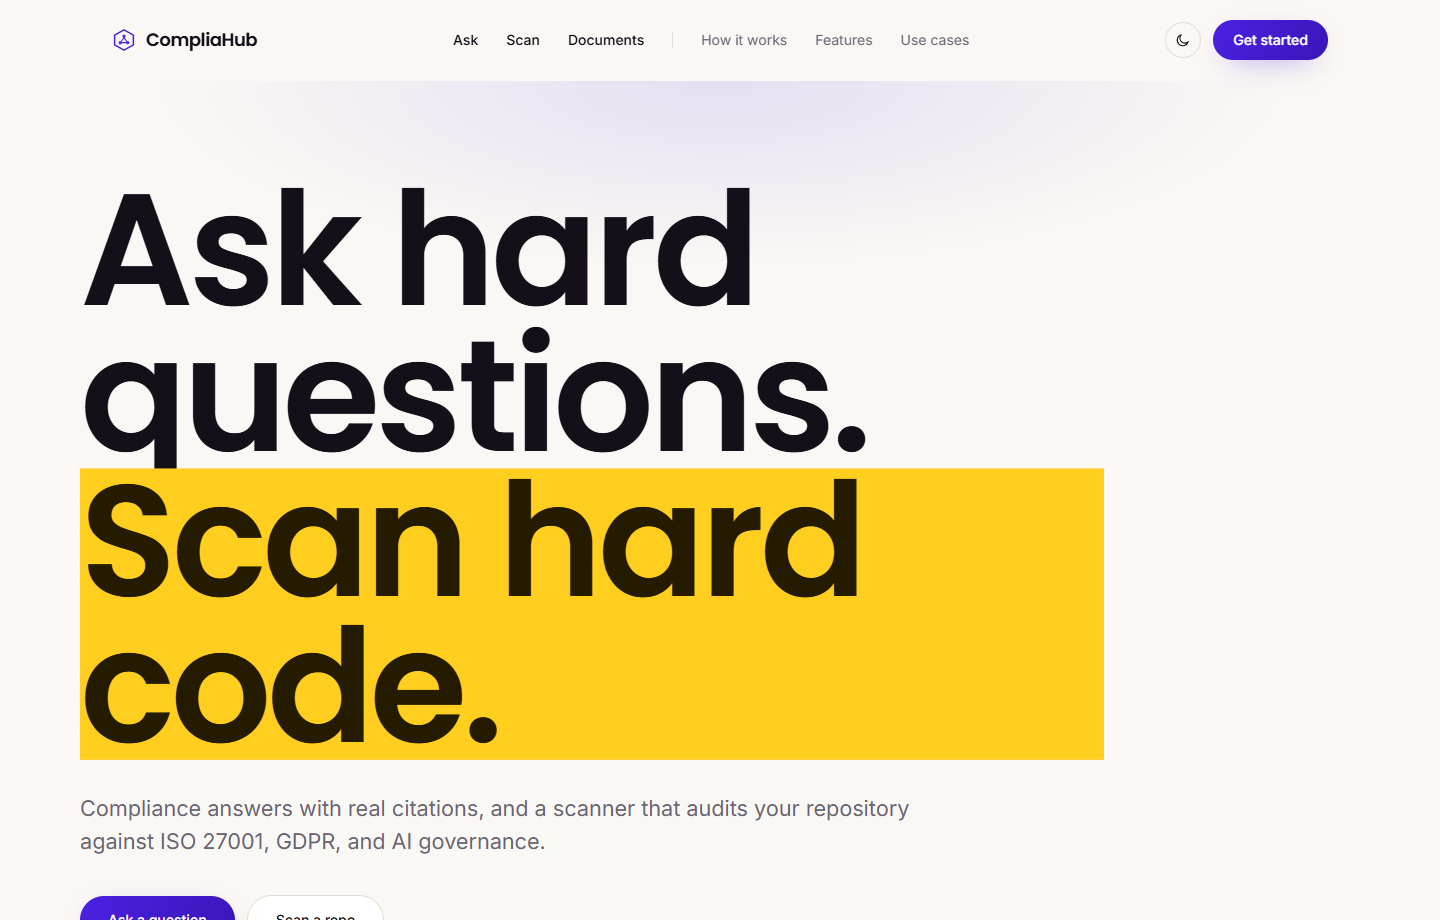
\includegraphics[width=0.95\textwidth]{images/screens/landing-light-hero.png}
\caption{Landing page: both product halves (Ask and Scan) discoverable from the home page}
\label{fig:ui-landing}
\end{figure}

\textbf{Chat (\texttt{/chat}, Figure~\ref{fig:ui-chat}).} The conversational
entry point to the \ac{RAG} layer. A question is classified into a routing
category and streamed back over \ac{SSE} token by token, so the answer is
visible as it is written rather than after a multi-second silent wait; each
claim in the answer carries one or more citation chips that, on click,
fetch and display the exact source passage they were grounded in. An empty
conversation greets the user with three example questions, each tagged with
the standard it maps to, so the range of questions the system can actually
answer is demonstrated rather than only described. Because only in-depth,
agent-routed questions persist a resumable thread on the backend, a
\emph{History} drawer lists past conversations by title and relative time,
reopens a resumable one, and explains -- rather than silently failing --
when a quick, non-agentic lookup has nothing to reopen. History is
device-local (no user accounts exist in this project), a limitation the
drawer discloses directly instead of hiding it.

\begin{figure}[H]
\centering
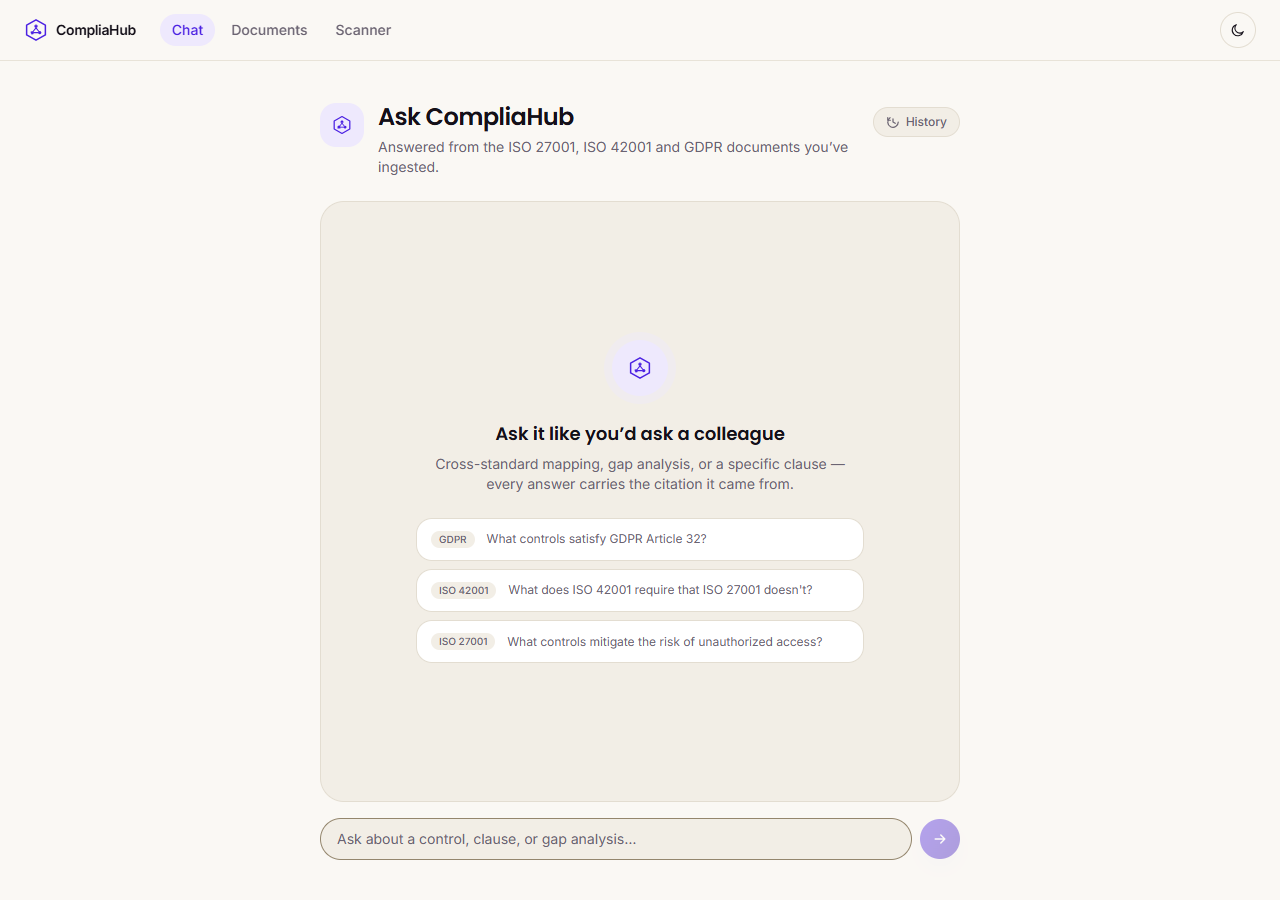
\includegraphics[width=0.8\textwidth]{images/screens/app-chat-light.png}
\caption{Conversational chat interface: an empty conversation with tagged example questions}
\label{fig:ui-chat}
\end{figure}

\textbf{Document ingestion (\texttt{/documents}, Figure~\ref{fig:ui-documents}).}
The entry point for the standards the chat and the scanner's AI-validation
pass both reason against. A drag-and-drop zone accepts a \ac{PDF} or DOCX
file and reflects, in real time, which stage of the ingestion pipeline
(parsing, chunking, embedding, graph extraction) is currently running for
each uploaded document; a failed stage surfaces its actual error message
rather than a generic failure state. Because no ``list every document''
endpoint exists on the backend, the page only ever tracks what was uploaded
in the current browser session -- a real, disclosed limitation of the
current \ac{API} rather than an oversight -- and says so directly in its
empty state.

\begin{figure}[H]
\centering
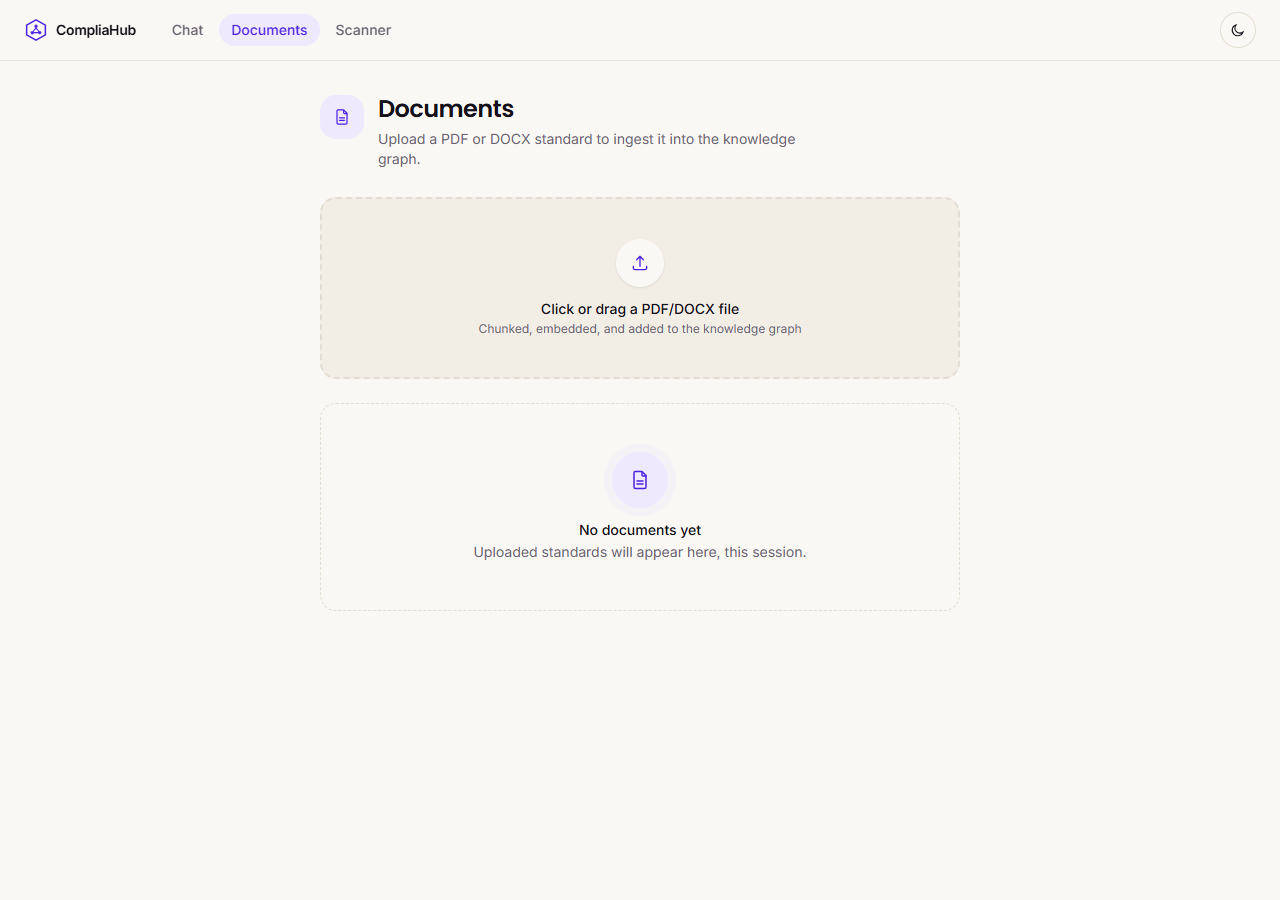
\includegraphics[width=0.8\textwidth]{images/screens/app-documents-light.png}
\caption{Document ingestion view: upload zone and empty-state messaging}
\label{fig:ui-documents}
\end{figure}

\textbf{Compliance Scanner.} The scanning half of the product spans three
screens that mirror the pipeline a repository actually goes through:
uploading it, watching its five analysis tracks run, and reading what they
found.

\emph{Repository list (\texttt{/scanner}, Figure~\ref{fig:ui-scanlist}).}
Symmetrical to the document-ingestion page, but for repository archives:
a drag-and-drop zone accepts a \texttt{.zip}, and -- unlike documents --
every past scan really is listed, since a \texttt{GET /scans} endpoint
exists on the backend, so scan history survives across browser sessions.
Each row summarizes a scan's file count, size, and detected languages, and
links through to that scan's detail view.

\begin{figure}[H]
\centering
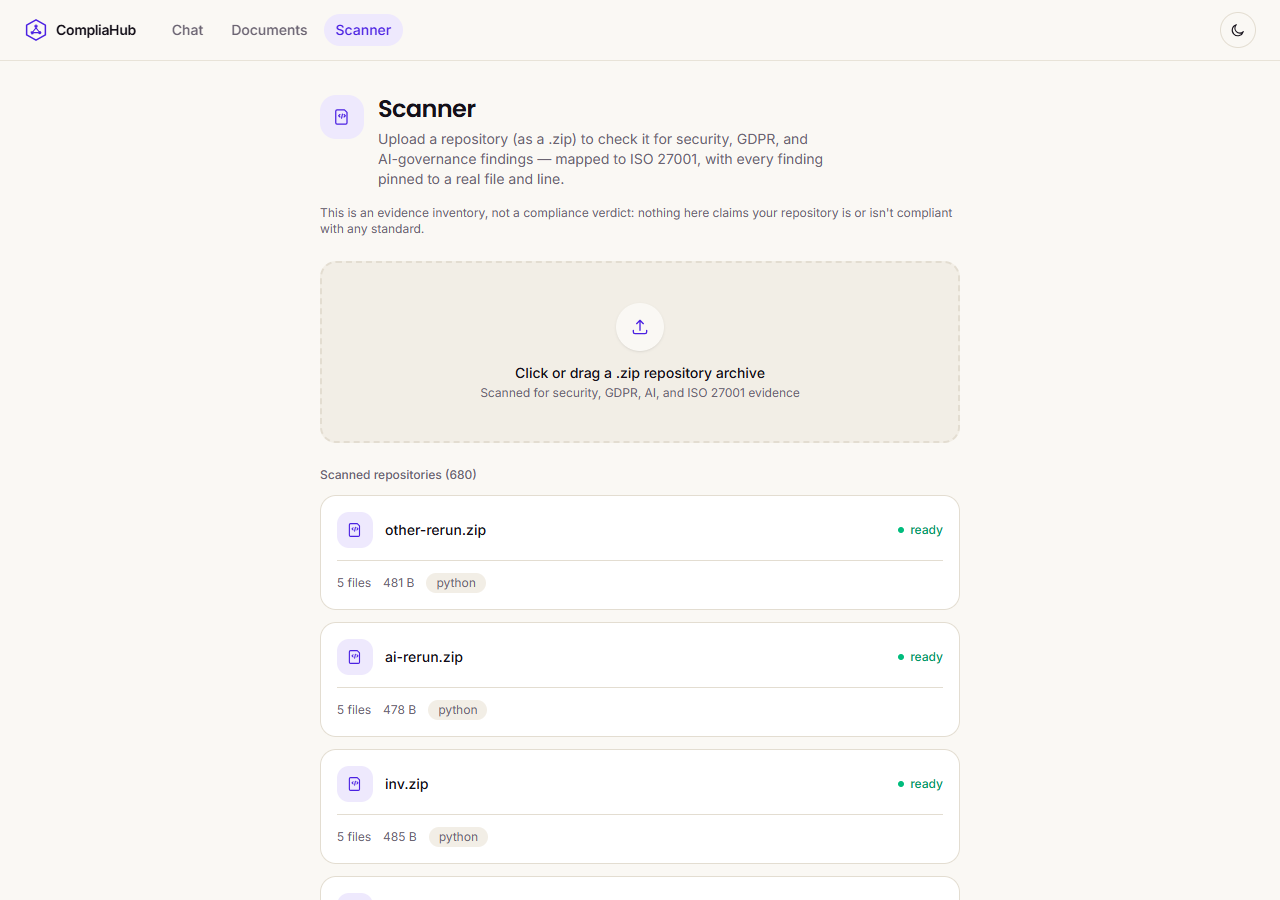
\includegraphics[width=0.95\textwidth]{images/screens/app-scanner-light.png}
\caption{Compliance Scanner: repository upload and scan history}
\label{fig:ui-scanlist}
\end{figure}

\emph{Scan detail (\texttt{/scanner/[scanId]}, Figure~\ref{fig:ui-scandetail}).}
The working view for a single scan. A five-stage pipeline tracker (extract,
security, \ac{GDPR}, AI/ISO 42001, ISO 27001) shows which of the scan's
independent analysis tracks have completed, are running, or have failed,
and a stat-card row summarizes files scanned, detected languages and
frameworks, and a findings-by-severity breakdown. Two tabs separate the raw
file inventory from the findings themselves; findings are filterable by
framework, review status, and a ``needs review only'' toggle, and each row
expands in place to show its full reasoning, its supporting evidence, two
actions -- triggering the agentic \ac{RAG} validation pass described in
Section~\ref{sec:code-description}, or requesting an automated unified-diff
remediation, neither of which can itself change the finding's status -- and
the human-review form itself (reviewer name, a decision, and a mandatory
written justification), the only mechanism in the system able to mark a
finding verified.

\begin{figure}[H]
\centering
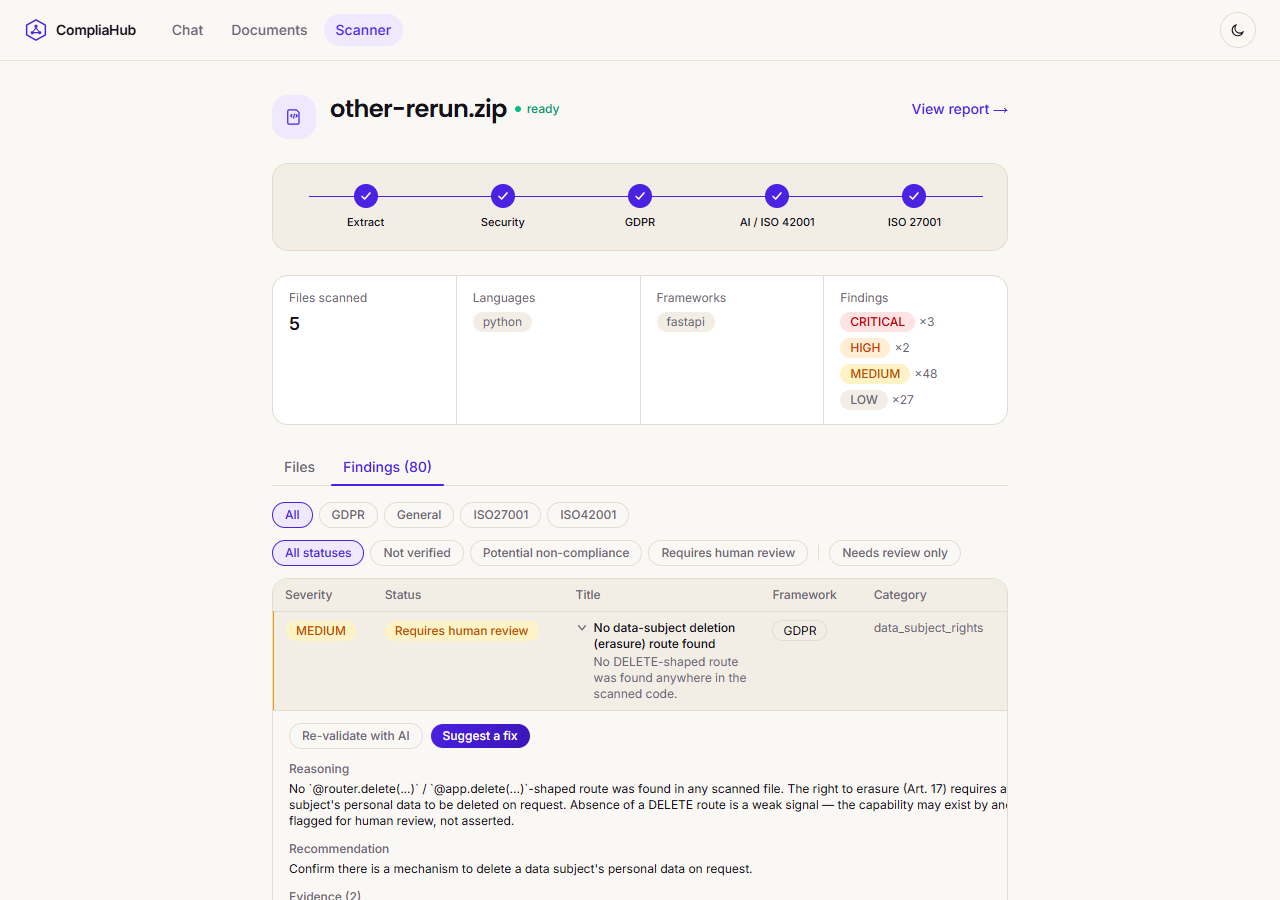
\includegraphics[width=0.95\textwidth]{images/screens/scan-detail-expanded-light.png}
\caption{Scan detail view: an expanded finding with AI validation/remediation and the human review form}
\label{fig:ui-scandetail}
\end{figure}

\emph{Evidence report (\texttt{/scanner/[scanId]/report}, Figure~\ref{fig:ui-report}).}
A single-page, printable artifact summarizing everything recorded against a
scan: stat cards for files, languages, and frameworks; three
findings-breakdown panels (by severity, by ISO 27001/GDPR/ISO 42001
framework, and by review status) rendered as proportional horizontal bars
rather than a bare table of numbers, each bar sized only against the
largest count \emph{within its own category} rather than against a total,
so that nothing on the page can be misread as a percentage; a human-review
coverage panel; and the full list of findings with their evidence and
review history. A standing disclaimer banner states plainly that the
report is technical evidence coverage, not a certification, audit opinion,
or compliance score -- a principle enforced in code by an automated test
that fails the build if any aggregate score-shaped string appears on the
page. Printing (or saving as \ac{PDF}) temporarily forces the light theme
regardless of which theme is active on screen, since a printed page must
not depend on a browser's dark-mode rendering of an on-screen report to
stay legible.

\begin{figure}[H]
\centering
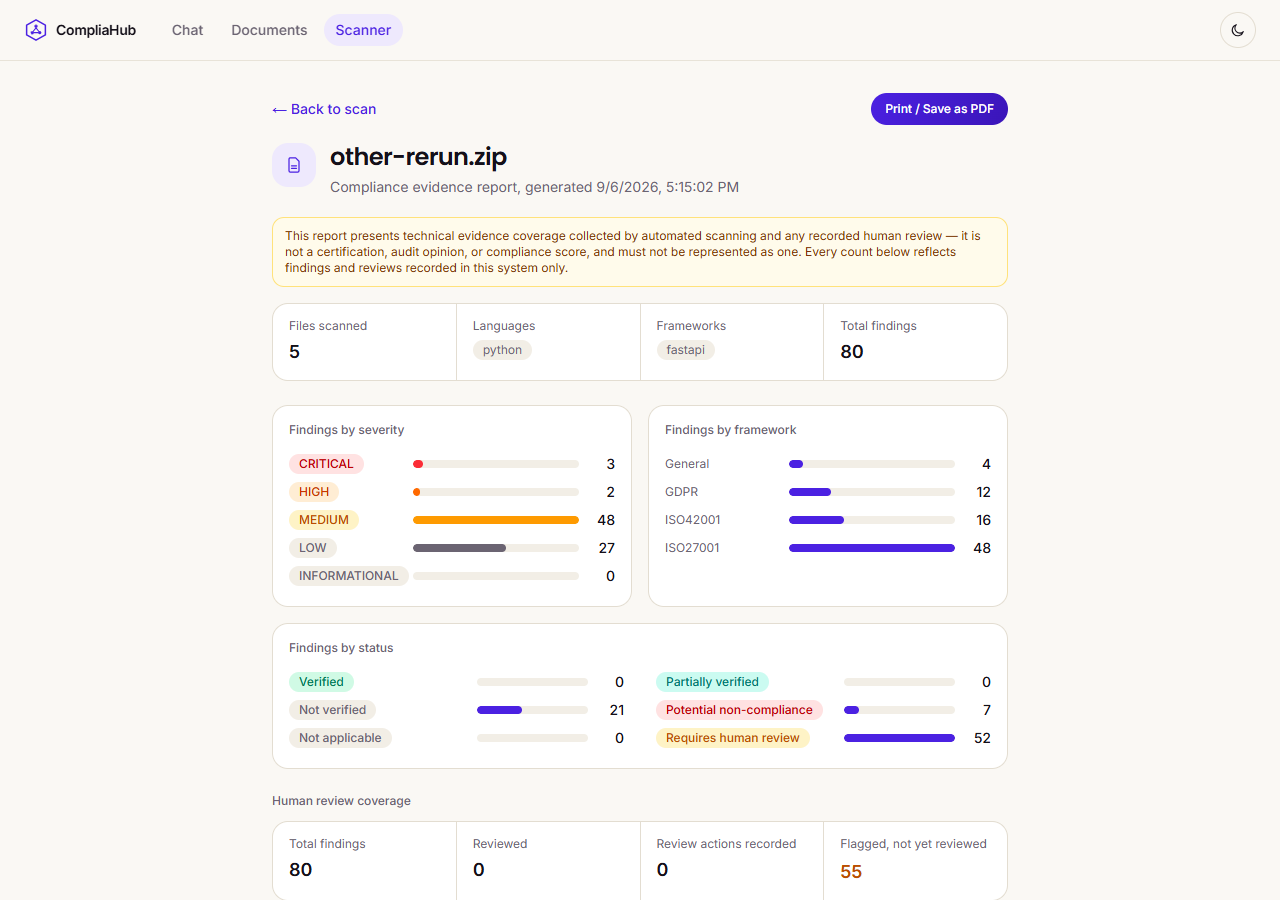
\includegraphics[width=0.95\textwidth]{images/screens/report-redesign.png}
\caption{Printable compliance evidence report: stat cards and severity/status/framework breakdowns}
\label{fig:ui-report}
\end{figure}

% ================================================================
% CHAPTER V -- TESTING AND VALIDATION
% ================================================================
\chapter{Tests et Validation}

\section{Test Methodology}

Testing followed two complementary layers throughout the project. On the
backend, \texttt{pytest} unit and integration tests were written alongside
every feature, but -- following an early, documented lesson of this project
-- every phase was additionally verified live against the real running
Docker stack (a real Postgres, Neo4j, Qdrant, Redis, MinIO, and Celery
workers), since mocked tests alone had previously missed real infrastructure
and hydration bugs. On the frontend, Playwright end-to-end tests run against
a genuine production build (\texttt{pnpm build} + \texttt{pnpm start}), not
the development server, because the development server had previously
masked a real hydration bug that only appeared in production. A dedicated
evaluation harness scores the conversational \ac{RAG} pipeline itself,
independent of ordinary unit testing, using a custom Gemini-based
\ac{LLM}-judge implementing the faithfulness, answer-relevance, context-
precision, and context-recall metrics.

\section{Test Cases and Results}

\begin{table}[H]
\centering
\caption{Test suite results at the end of the internship}
\label{tab:testresults}
\begin{tabularx}{\textwidth}{@{}l X@{}}
\toprule
\textbf{Suite} & \textbf{Result} \\
\midrule
Backend (\texttt{pytest}) & 511 passed, 0 failed, 0 skipped; \texttt{ruff} clean \\
Frontend (Playwright, end-to-end) & 37 passed -- landing page, hero-animation timing, live chat streaming against the real backend, scan-detail interactions, printable-report content, \ac{WCAG} contrast, and accessibility sweeps across all six routes \\
Automated remediation unit tests & 19 passed (11 remediation-flow + 8 diff-generation tests, including the trailing-newline regression) \\
Evaluation harness (live run) & 1 question scored: faithfulness = 1.00, answer relevance $\approx$ 0.79, context precision = 1.00, context recall = 1.00 \\
\bottomrule
\end{tabularx}
\end{table}

A second evaluation question in the same live run hit a transient DNS
resolution error; the error was correctly isolated to that single question's
own result row without failing the rest of the run, and the question
succeeded cleanly on a retry -- confirming the harness's per-question error
isolation works in practice, not only in a unit test.

\section{Performance Analysis}

Latency was not benchmarked in isolation with a dedicated load-testing tool
within the timeframe of this internship; the figures available are
browser-observed, end-to-end timings taken from live Playwright runs (which
include page load, hydration, and network round-trip, not a pure server-side
measurement), and are reported here as such rather than as an isolated
backend latency claim. A dedicated ingestion load test at the originally
planned scale (100--300 documents) was deliberately scaled back to a single
real document, for two independently discovered and disclosed reasons: the
shared development database's own accumulated 311-document test-pollution
(see Chapter~IV), and repeated out-of-memory conditions on the development
machine while multiple unrelated Docker projects competed for the same
memory budget. Both are recorded as explicit, open follow-ups rather than
silently glossed over.

\section{Comparison with the Original Non-Functional Objectives}

\begin{table}[H]
\centering
\caption{Non-functional objectives vs. verification status}
\label{tab:nfrcheck}
\begin{tabularx}{\textwidth}{@{}l X l@{}}
\toprule
\textbf{Objective} & \textbf{Verification method} & \textbf{Status} \\
\midrule
Cited, multi-hop answers & Manual review + live queries & Met \\
Security (API key + rate limit) & Unit tests + live request checks & Met \\
\ac{WCAG} AA contrast & Automated computed-style test & Met \\
Reduced-motion support & Automated \& manual review & Met \\
Print-fidelity of the report & Manual print-preview verification & Met \\
Incremental ingestion & Implemented; full-corpus rebuild cost & Partially verified \\
 & at real (311-document) scale not load-tested & (disclosed gap) \\
Load-test at planned scale & Script built, scope reduced (see above) & Deferred \\
\bottomrule
\end{tabularx}
\end{table}

% ================================================================
% CHAPTER VI -- CONCLUSION
% ================================================================
\chapter{Conclusion and Perspectives}

\section{Project Summary}

Over the course of a two-month internship, the CompliaHub platform was
designed, implemented, and validated end to end: an agentic GraphRAG
compliance-intelligence engine spanning ingestion, vector and graph
retrieval, and multi-step agent orchestration; a Compliance Scanner reusing
that same infrastructure to turn a source-code repository into
evidence-grounded, human-verified compliance findings mapped to ISO 27001
Annex A; and a redesigned, accessible, dual-theme frontend surfacing both
halves of the product. All 18 phases of the original two-track roadmap were
completed and live-verified, backed by 511 passing backend tests and 37
passing end-to-end frontend tests at the time of writing.

\section{Personal and Technical Contributions}

This internship provided hands-on experience across the full depth of a
modern \ac{RAG} system: designing and operating a polyglot persistence layer
(relational, vector, and graph stores); building a stateful, multi-step
agent with LangGraph; building a fully custom \ac{LLM}-judge evaluation
harness rather than adopting an existing library, deliberately, to
understand every metric's computation from first principles; designing an
accessible, \ac{WCAG}-compliant, dual-theme frontend with automated
regression tests for both contrast and keyboard operability; and operating
a disciplined, documentation-first, live-verified development methodology
across an unusually large, 18-phase solo project.

\section{Possible Improvements and Perspectives}

\begin{itemize}
  \item \textbf{Graph sharding at scale.} A concrete sharding strategy
        (per-standard partitioning, with the existing \texttt{MAPS\_TO}
        relation as the required cross-shard bridge) is already documented
        but was deliberately not implemented, since the current corpus size
        does not yet justify it -- a clear, actionable next step once real
        usage crosses the documented trigger thresholds.
  \item \textbf{Load testing at realistic scale}, once the shared
        development database's accumulated test-pollution is cleaned up and
        on a machine with adequate memory headroom.
  \item \textbf{Broader ISO 27001 Annex A coverage}, extending the current
        Technological (A.8) and partial Organizational (A.5) control
        mapping to the People and Physical control families.
  \item \textbf{Dedicated observability tooling} (e.g. Langfuse-style
        tracing), explicitly deferred in favor of the current
        structured-logging approach while the system operates at its
        present scale, and a natural next investment if usage grows.
  \item \textbf{Multilingual document support}, an explicit non-goal of
        this first version, would extend the platform's applicability
        beyond English-language standards.
\end{itemize}

% ================================================================
% ANNEXES
% ================================================================
\renewcommand{\thechapter}{\Alph{chapter}}
\setcounter{chapter}{0}

\chapter{Selected Backend API Endpoints}

\begin{table}[H]
\centering
\caption{Selected backend API endpoints}
\label{tab:endpoints}
\begin{tabularx}{\textwidth}{@{}l X@{}}
\toprule
\textbf{Endpoint} & \textbf{Purpose} \\
\midrule
\texttt{GET /health}, \texttt{/health/deep} & Liveness and per-service connectivity check \\
\texttt{POST /documents} & Upload a \ac{PDF}/DOCX for ingestion \\
\texttt{DELETE /documents/\{id\}} & Remove a document and rebuild the entity graph \\
\texttt{POST /query}, \texttt{/query/stream} & Ask a question (synchronous or \ac{SSE} streaming) \\
\texttt{GET /query/conversations/\{id\}} & Inspect a multi-turn agent conversation \\
\texttt{POST /scans} & Upload a repository \texttt{.zip} to the scanner \\
\texttt{GET /scans/\{id\}/findings} & List a scan's findings \\
\texttt{POST /scans/\{id\}/findings/\{fid\}/validate} & Trigger AI validation of a finding \\
\texttt{POST /scans/\{id\}/findings/\{fid\}/remediate} & Trigger AI remediation-diff suggestion \\
\texttt{POST /scans/\{id\}/findings/\{fid\}/reviews} & Submit a human review \\
\texttt{GET /scans/\{id\}/summary} & Printable-report summary data \\
\texttt{POST /eval/runs} & Run the evaluation harness \\
\bottomrule
\end{tabularx}
\end{table}

\chapter{Illustrative Control-Status Decision Logic}

The following is a simplified, illustrative pseudocode representation of
the control-status decision logic described in Chapter~IV -- not a verbatim
source excerpt, but a faithful summary of the actual decision rule.

\begin{lstlisting}[language=Python, caption={Illustrative control-status decision logic}]
def decide_control_status(automatable, mapped_findings):
    if not automatable:
        return "REQUIRES_HUMAN_REVIEW"
    if not mapped_findings:
        return "NOT_VERIFIED"
    if all(f.status == "REQUIRES_HUMAN_REVIEW" for f in mapped_findings):
        return "REQUIRES_HUMAN_REVIEW"
    # Positive resolution still requires a recorded human review
    # on every mapped finding before the control itself can be
    # marked VERIFIED / PARTIALLY_VERIFIED.
    return aggregate_with_max_severity(mapped_findings)
\end{lstlisting}

\chapter{Compliance Scanner Pipeline}

\begin{figure}[H]
\centering
\begin{tikzpicture}[
  step/.style={draw, rectangle, rounded corners, minimum width=2.1cm, minimum height=1cm, align=center, font=\footnotesize},
  >=Latex
]
  \node[step] (s1) at (0,0)    {1. Upload};
  \node[step] (s2) at (2.4,0)  {2. Scan};
  \node[step] (s3) at (4.8,0)  {3. Map};
  \node[step] (s4) at (7.2,0)  {4. Validate};
  \node[step] (s5) at (9.6,0)  {5. Remediate};
  \node[step] (s6) at (12.0,0) {6. Review};
  \node[step] (s7) at (14.4,0) {7. Report};

  \draw[->] (s1) -- (s2);
  \draw[->] (s2) -- (s3);
  \draw[->] (s3) -- (s4);
  \draw[->] (s4) -- (s5);
  \draw[->] (s5) -- (s6);
  \draw[->] (s6) -- (s7);
\end{tikzpicture}
\caption{The Compliance Scanner's seven-step pipeline}
\label{fig:scannerpipeline}
\end{figure}

Only step 6 (Review) can move a finding to a positive status; steps 1--5 and
7 never assert compliance on their own.

% ================================================================
% BIBLIOGRAPHY
% ================================================================
\begin{thebibliography}{99}
\addcontentsline{toc}{chapter}{Bibliography}

\bibitem{edge2024graphrag}
D. Edge, H. Trinh, N. Cheng, J. Bradley, A. Chao, A. Mody, S. Truitt, and
J. Larson, ``From Local to Global: A Graph RAG Approach to Query-Focused
Summarization,'' \emph{arXiv preprint arXiv:2404.16130}, 2024.

\bibitem{fastapi}
FastAPI, ``FastAPI Documentation,'' \url{https://fastapi.tiangolo.com/}.

\bibitem{nextjs}
Vercel, ``Next.js Documentation,'' \url{https://nextjs.org/docs}.

\bibitem{neo4j}
Neo4j, Inc., ``Neo4j Graph Database Documentation,'' \url{https://neo4j.com/docs/}.

\bibitem{qdrant}
Qdrant, ``Qdrant Vector Database Documentation,'' \url{https://qdrant.tech/documentation/}.

\bibitem{langgraph}
LangChain, ``LangGraph Documentation,'' \url{https://langchain-ai.github.io/langgraph/}.

\bibitem{docling}
IBM Research, ``Docling: Document Conversion Toolkit,'' \url{https://github.com/DS4SD/docling}.

\bibitem{voyageai}
Voyage AI, ``Voyage AI Embeddings Documentation,'' \url{https://docs.voyageai.com/}.

\bibitem{cohere}
Cohere, ``Cohere Rerank Documentation,'' \url{https://docs.cohere.com/docs/rerank}.

\bibitem{gemini}
Google, ``Gemini API Documentation,'' \url{https://ai.google.dev/gemini-api/docs}.

\bibitem{ragas}
S. Es, J. James, L. Espinosa-Anke, and S. Schockaert, ``RAGAS: Automated
Evaluation of Retrieval Augmented Generation,'' \emph{arXiv preprint
arXiv:2309.15217}, 2023.

\bibitem{iso27001}
International Organization for Standardization, ``ISO/IEC 27001:2022 --
Information Security, Cybersecurity and Privacy Protection -- Information
Security Management Systems -- Requirements.''

\bibitem{iso42001}
International Organization for Standardization, ``ISO/IEC 42001:2023 --
Information Technology -- Artificial Intelligence -- Management System.''

\bibitem{gdpr}
European Parliament and Council of the European Union, ``Regulation (EU)
2016/679 (General Data Protection Regulation),'' Official Journal of the
European Union, 2016.

\bibitem{wcag}
W3C, ``Web Content Accessibility Guidelines (WCAG) 2.1,''
\url{https://www.w3.org/TR/WCAG21/}.

\bibitem{vercel}
Vercel Inc., ``Vercel Deployment Documentation,'' \url{https://vercel.com/docs}.

\bibitem{docker}
Docker Inc., ``Docker Compose Documentation,'' \url{https://docs.docker.com/compose/}.

\end{thebibliography}

\end{document}
